\documentclass[twoside]{book}

% Packages required by doxygen
\usepackage{fixltx2e}
\usepackage{calc}
\usepackage{doxygen}
\usepackage[export]{adjustbox} % also loads graphicx
\usepackage{graphicx}
\usepackage[utf8]{inputenc}
\usepackage{makeidx}
\usepackage{multicol}
\usepackage{multirow}
\PassOptionsToPackage{warn}{textcomp}
\usepackage{textcomp}
\usepackage[nointegrals]{wasysym}
\usepackage[table]{xcolor}

% Font selection
\usepackage[T1]{fontenc}
\usepackage[scaled=.90]{helvet}
\usepackage{courier}
\usepackage{amssymb}
\usepackage{sectsty}
\renewcommand{\familydefault}{\sfdefault}
\allsectionsfont{%
  \fontseries{bc}\selectfont%
  \color{darkgray}%
}
\renewcommand{\DoxyLabelFont}{%
  \fontseries{bc}\selectfont%
  \color{darkgray}%
}
\newcommand{\+}{\discretionary{\mbox{\scriptsize$\hookleftarrow$}}{}{}}

% Page & text layout
\usepackage{geometry}
\geometry{%
  a4paper,%
  top=2.5cm,%
  bottom=2.5cm,%
  left=2.5cm,%
  right=2.5cm%
}
\tolerance=750
\hfuzz=15pt
\hbadness=750
\setlength{\emergencystretch}{15pt}
\setlength{\parindent}{0cm}
\setlength{\parskip}{3ex plus 2ex minus 2ex}
\makeatletter
\renewcommand{\paragraph}{%
  \@startsection{paragraph}{4}{0ex}{-1.0ex}{1.0ex}{%
    \normalfont\normalsize\bfseries\SS@parafont%
  }%
}
\renewcommand{\subparagraph}{%
  \@startsection{subparagraph}{5}{0ex}{-1.0ex}{1.0ex}{%
    \normalfont\normalsize\bfseries\SS@subparafont%
  }%
}
\makeatother

% Headers & footers
\usepackage{fancyhdr}
\pagestyle{fancyplain}
\fancyhead[LE]{\fancyplain{}{\bfseries\thepage}}
\fancyhead[CE]{\fancyplain{}{}}
\fancyhead[RE]{\fancyplain{}{\bfseries\leftmark}}
\fancyhead[LO]{\fancyplain{}{\bfseries\rightmark}}
\fancyhead[CO]{\fancyplain{}{}}
\fancyhead[RO]{\fancyplain{}{\bfseries\thepage}}
\fancyfoot[LE]{\fancyplain{}{}}
\fancyfoot[CE]{\fancyplain{}{}}
\fancyfoot[RE]{\fancyplain{}{\bfseries\scriptsize Generated by Doxygen }}
\fancyfoot[LO]{\fancyplain{}{\bfseries\scriptsize Generated by Doxygen }}
\fancyfoot[CO]{\fancyplain{}{}}
\fancyfoot[RO]{\fancyplain{}{}}
\renewcommand{\footrulewidth}{0.4pt}
\renewcommand{\chaptermark}[1]{%
  \markboth{#1}{}%
}
\renewcommand{\sectionmark}[1]{%
  \markright{\thesection\ #1}%
}

% Indices & bibliography
\usepackage{natbib}
\usepackage[titles]{tocloft}
\setcounter{tocdepth}{3}
\setcounter{secnumdepth}{5}
\makeindex

% Hyperlinks (required, but should be loaded last)
\usepackage{ifpdf}
\ifpdf
  \usepackage[pdftex,pagebackref=true]{hyperref}
\else
  \usepackage[ps2pdf,pagebackref=true]{hyperref}
\fi
\hypersetup{%
  colorlinks=true,%
  linkcolor=blue,%
  citecolor=blue,%
  unicode%
}

% Custom commands
\newcommand{\clearemptydoublepage}{%
  \newpage{\pagestyle{empty}\cleardoublepage}%
}

\usepackage{caption}
\captionsetup{labelsep=space,justification=centering,font={bf},singlelinecheck=off,skip=4pt,position=top}

%===== C O N T E N T S =====

\begin{document}

% Titlepage & ToC
\hypersetup{pageanchor=false,
             bookmarksnumbered=true,
             pdfencoding=unicode
            }
\pagenumbering{alph}
\begin{titlepage}
\vspace*{7cm}
\begin{center}%
{\Large My Project }\\
\vspace*{1cm}
{\large Generated by Doxygen 1.8.13}\\
\end{center}
\end{titlepage}
\clearemptydoublepage
\pagenumbering{roman}
\tableofcontents
\clearemptydoublepage
\pagenumbering{arabic}
\hypersetup{pageanchor=true}

%--- Begin generated contents ---
\chapter{Class Index}
\section{Class List}
Here are the classes, structs, unions and interfaces with brief descriptions\+:\begin{DoxyCompactList}
\item\contentsline{section}{\hyperlink{structCOORDENADA}{C\+O\+O\+R\+D\+E\+N\+A\+DA} }{\pageref{structCOORDENADA}}{}
\item\contentsline{section}{\hyperlink{structESTADO}{E\+S\+T\+A\+DO} \\*Definição do estado }{\pageref{structESTADO}}{}
\item\contentsline{section}{\hyperlink{structJOGADA}{J\+O\+G\+A\+DA} \\*Definição da jogada }{\pageref{structJOGADA}}{}
\end{DoxyCompactList}

\chapter{File Index}
\section{File List}
Here is a list of all documented files with brief descriptions\+:\begin{DoxyCompactList}
\item\contentsline{section}{\hyperlink{camada__da__interface_8h}{camada\+\_\+da\+\_\+interface.\+h} }{\pageref{camada__da__interface_8h}}{}
\item\contentsline{section}{\hyperlink{camada__de__dados_8h}{camada\+\_\+de\+\_\+dados.\+h} }{\pageref{camada__de__dados_8h}}{}
\item\contentsline{section}{\hyperlink{logica__do__programa_8h}{logica\+\_\+do\+\_\+programa.\+h} }{\pageref{logica__do__programa_8h}}{}
\item\contentsline{section}{\hyperlink{main_8c}{main.\+c} }{\pageref{main_8c}}{}
\end{DoxyCompactList}

\chapter{Class Documentation}
\hypertarget{structCOORDENADA}{}\section{C\+O\+O\+R\+D\+E\+N\+A\+DA Struct Reference}
\label{structCOORDENADA}\index{C\+O\+O\+R\+D\+E\+N\+A\+DA@{C\+O\+O\+R\+D\+E\+N\+A\+DA}}
\subsection*{Public Attributes}
\begin{DoxyCompactItemize}
\item 
\mbox{\Hypertarget{structCOORDENADA_adfbc8d4856ce807139fdf62e00aed29a}\label{structCOORDENADA_adfbc8d4856ce807139fdf62e00aed29a}} 
int {\bfseries coluna}
\item 
\mbox{\Hypertarget{structCOORDENADA_aefe14bcc5a066ac3b21500cc3d28c06f}\label{structCOORDENADA_aefe14bcc5a066ac3b21500cc3d28c06f}} 
int {\bfseries linha}
\end{DoxyCompactItemize}


The documentation for this struct was generated from the following file\+:\begin{DoxyCompactItemize}
\item 
\hyperlink{camada__de__dados_8h}{camada\+\_\+de\+\_\+dados.\+h}\end{DoxyCompactItemize}

\hypertarget{structESTADO}{}\section{E\+S\+T\+A\+DO Struct Reference}
\label{structESTADO}\index{E\+S\+T\+A\+DO@{E\+S\+T\+A\+DO}}


Definição do estado.  




{\ttfamily \#include $<$camada\+\_\+de\+\_\+dados.\+h$>$}



Collaboration diagram for E\+S\+T\+A\+DO\+:
\nopagebreak
\begin{figure}[H]
\begin{center}
\leavevmode
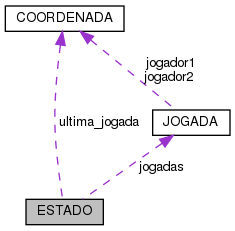
\includegraphics[width=249pt]{structESTADO__coll__graph}
\end{center}
\end{figure}
\subsection*{Public Attributes}
\begin{DoxyCompactItemize}
\item 
\mbox{\Hypertarget{structESTADO_ab56f0f1be16954d3768b4174d14c087d}\label{structESTADO_ab56f0f1be16954d3768b4174d14c087d}} 
\hyperlink{camada__de__dados_8h_aba91601f16d4c485b2d9b8c429f27039}{C\+A\+SA} {\bfseries tab} \mbox{[}8\mbox{]}\mbox{[}8\mbox{]}
\item 
\mbox{\Hypertarget{structESTADO_a4896a5c5c1f40b43fb795623327e3f47}\label{structESTADO_a4896a5c5c1f40b43fb795623327e3f47}} 
\hyperlink{structCOORDENADA}{C\+O\+O\+R\+D\+E\+N\+A\+DA} {\bfseries ultima\+\_\+jogada}
\item 
\mbox{\Hypertarget{structESTADO_afae43b87a488fad0f2b56a18bad31d18}\label{structESTADO_afae43b87a488fad0f2b56a18bad31d18}} 
J\+O\+G\+A\+D\+AS {\bfseries jogadas}
\item 
\mbox{\Hypertarget{structESTADO_a261495728744647e618b4e623f5a4b7a}\label{structESTADO_a261495728744647e618b4e623f5a4b7a}} 
int {\bfseries num\+\_\+jogadas}
\item 
\mbox{\Hypertarget{structESTADO_a5dd28e2e68b7aef2b6b7ea88e02eff58}\label{structESTADO_a5dd28e2e68b7aef2b6b7ea88e02eff58}} 
int {\bfseries jogador\+\_\+atual}
\end{DoxyCompactItemize}


\subsection{Detailed Description}
Definição do estado. 

The documentation for this struct was generated from the following file\+:\begin{DoxyCompactItemize}
\item 
\hyperlink{camada__de__dados_8h}{camada\+\_\+de\+\_\+dados.\+h}\end{DoxyCompactItemize}

\hypertarget{structJOGADA}{}\section{J\+O\+G\+A\+DA Struct Reference}
\label{structJOGADA}\index{J\+O\+G\+A\+DA@{J\+O\+G\+A\+DA}}


Definição da jogada.  




{\ttfamily \#include $<$camada\+\_\+de\+\_\+dados.\+h$>$}



Collaboration diagram for J\+O\+G\+A\+DA\+:
\nopagebreak
\begin{figure}[H]
\begin{center}
\leavevmode
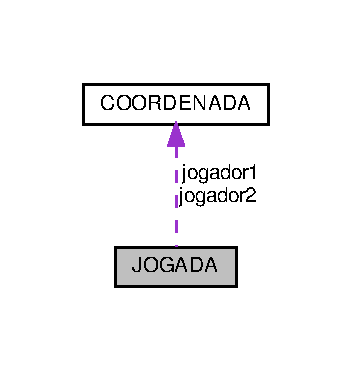
\includegraphics[width=169pt]{structJOGADA__coll__graph}
\end{center}
\end{figure}
\subsection*{Public Attributes}
\begin{DoxyCompactItemize}
\item 
\mbox{\Hypertarget{structJOGADA_a93d9306cb0c49b66b7d9a615bffe0149}\label{structJOGADA_a93d9306cb0c49b66b7d9a615bffe0149}} 
\hyperlink{structCOORDENADA}{C\+O\+O\+R\+D\+E\+N\+A\+DA} {\bfseries jogador1}
\item 
\mbox{\Hypertarget{structJOGADA_ab46b16dfbdc7f2af9430c8dcdac0914b}\label{structJOGADA_ab46b16dfbdc7f2af9430c8dcdac0914b}} 
\hyperlink{structCOORDENADA}{C\+O\+O\+R\+D\+E\+N\+A\+DA} {\bfseries jogador2}
\end{DoxyCompactItemize}


\subsection{Detailed Description}
Definição da jogada. 

The documentation for this struct was generated from the following file\+:\begin{DoxyCompactItemize}
\item 
\hyperlink{camada__de__dados_8h}{camada\+\_\+de\+\_\+dados.\+h}\end{DoxyCompactItemize}

\chapter{File Documentation}
\hypertarget{camada__da__interface_8h}{}\section{camada\+\_\+da\+\_\+interface.\+h File Reference}
\label{camada__da__interface_8h}\index{camada\+\_\+da\+\_\+interface.\+h@{camada\+\_\+da\+\_\+interface.\+h}}
{\ttfamily \#include \char`\"{}camada\+\_\+de\+\_\+dados.\+h\char`\"{}}\newline
{\ttfamily \#include \char`\"{}logica\+\_\+do\+\_\+programa.\+h\char`\"{}}\newline
{\ttfamily \#include \char`\"{}camada\+\_\+da\+\_\+interface.\+h\char`\"{}}\newline
Include dependency graph for camada\+\_\+da\+\_\+interface.\+h\+:
\nopagebreak
\begin{figure}[H]
\begin{center}
\leavevmode
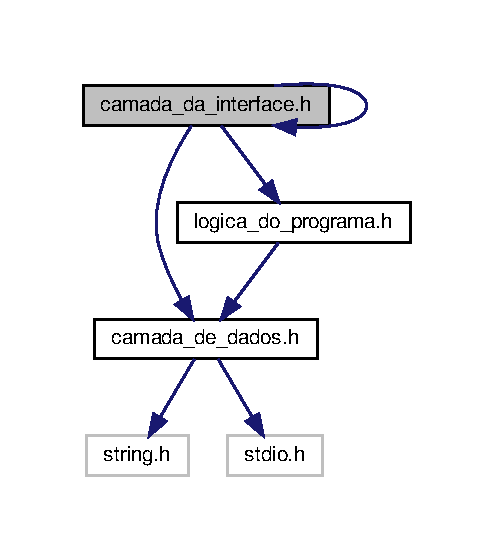
\includegraphics[width=237pt]{camada__da__interface_8h__incl}
\end{center}
\end{figure}
This graph shows which files directly or indirectly include this file\+:
\nopagebreak
\begin{figure}[H]
\begin{center}
\leavevmode
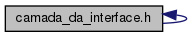
\includegraphics[width=216pt]{camada__da__interface_8h__dep__incl}
\end{center}
\end{figure}
\subsection*{Functions}
\begin{DoxyCompactItemize}
\item 
\mbox{\Hypertarget{camada__da__interface_8h_a4525a57d0cd9ed3c9150e19b67e1dad6}\label{camada__da__interface_8h_a4525a57d0cd9ed3c9150e19b67e1dad6}} 
void \hyperlink{camada__da__interface_8h_a4525a57d0cd9ed3c9150e19b67e1dad6}{mostrar\+\_\+tabuleiro} (\hyperlink{structESTADO}{E\+S\+T\+A\+DO} $\ast$estado)
\begin{DoxyCompactList}\small\item\em Função que desenha o tabuleiro no estado atual. \end{DoxyCompactList}\item 
\mbox{\Hypertarget{camada__da__interface_8h_a3cec1f7f711da0874ec656837ad771fe}\label{camada__da__interface_8h_a3cec1f7f711da0874ec656837ad771fe}} 
void \hyperlink{camada__da__interface_8h_a3cec1f7f711da0874ec656837ad771fe}{escreve\+\_\+tabuleuiro} (\hyperlink{structESTADO}{E\+S\+T\+A\+DO} $\ast$e, F\+I\+LE $\ast$save)
\begin{DoxyCompactList}\small\item\em Função auxiliar da função gravar\+\_\+estado. \end{DoxyCompactList}\item 
\mbox{\Hypertarget{camada__da__interface_8h_aa4d2bacf7b2ab01ba45b8dd7467a4cac}\label{camada__da__interface_8h_aa4d2bacf7b2ab01ba45b8dd7467a4cac}} 
void \hyperlink{camada__da__interface_8h_aa4d2bacf7b2ab01ba45b8dd7467a4cac}{gravar\+\_\+estado} (\hyperlink{structESTADO}{E\+S\+T\+A\+DO} $\ast$e, char filename\mbox{[}$\,$\mbox{]})
\begin{DoxyCompactList}\small\item\em Função auxiliar da função interpretador que escreve um estado em um ficheiro. \end{DoxyCompactList}\item 
\mbox{\Hypertarget{camada__da__interface_8h_adce9ef003e0e006df5b8bbb186111aff}\label{camada__da__interface_8h_adce9ef003e0e006df5b8bbb186111aff}} 
void \hyperlink{camada__da__interface_8h_adce9ef003e0e006df5b8bbb186111aff}{ler\+\_\+estado} (char filename\mbox{[}$\,$\mbox{]})
\begin{DoxyCompactList}\small\item\em Função que lê o estado de um ficheiro. \end{DoxyCompactList}\item 
\mbox{\Hypertarget{camada__da__interface_8h_a24da95ebeede4a540e37790ce8be359b}\label{camada__da__interface_8h_a24da95ebeede4a540e37790ce8be359b}} 
int \hyperlink{camada__da__interface_8h_a24da95ebeede4a540e37790ce8be359b}{interpretador} (\hyperlink{structESTADO}{E\+S\+T\+A\+DO} $\ast$e)
\begin{DoxyCompactList}\small\item\em Função que tranforma comandos dos jogador em ações no estado do jogo. \end{DoxyCompactList}\item 
\mbox{\Hypertarget{camada__da__interface_8h_ae41fb376b5e99f2c6981f8c754806bfe}\label{camada__da__interface_8h_ae41fb376b5e99f2c6981f8c754806bfe}} 
char \hyperlink{camada__da__interface_8h_ae41fb376b5e99f2c6981f8c754806bfe}{letra} (int x)
\begin{DoxyCompactList}\small\item\em Função auxiliar da função void que tranforma um número na sua letra logicamente correspondente. \end{DoxyCompactList}\item 
\mbox{\Hypertarget{camada__da__interface_8h_a33d09196f922a638847c19f3aca3fc3c}\label{camada__da__interface_8h_a33d09196f922a638847c19f3aca3fc3c}} 
void \hyperlink{camada__da__interface_8h_a33d09196f922a638847c19f3aca3fc3c}{prompt} (\hyperlink{structESTADO}{E\+S\+T\+A\+DO} $\ast$e)
\begin{DoxyCompactList}\small\item\em Função que fornece informação sobre o estado do jogo aos jogadores. \end{DoxyCompactList}\end{DoxyCompactItemize}


\subsection{Detailed Description}
Definição das funções relacionadas com interface 
\hypertarget{camada__de__dados_8h}{}\section{camada\+\_\+de\+\_\+dados.\+h File Reference}
\label{camada__de__dados_8h}\index{camada\+\_\+de\+\_\+dados.\+h@{camada\+\_\+de\+\_\+dados.\+h}}
{\ttfamily \#include $<$string.\+h$>$}\newline
{\ttfamily \#include $<$stdio.\+h$>$}\newline
Include dependency graph for camada\+\_\+de\+\_\+dados.\+h\+:
\nopagebreak
\begin{figure}[H]
\begin{center}
\leavevmode
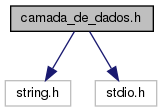
\includegraphics[width=194pt]{camada__de__dados_8h__incl}
\end{center}
\end{figure}
This graph shows which files directly or indirectly include this file\+:
\nopagebreak
\begin{figure}[H]
\begin{center}
\leavevmode
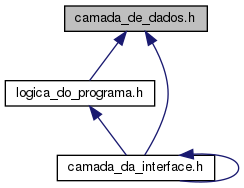
\includegraphics[width=255pt]{camada__de__dados_8h__dep__incl}
\end{center}
\end{figure}
\subsection*{Classes}
\begin{DoxyCompactItemize}
\item 
struct \hyperlink{structCOORDENADA}{C\+O\+O\+R\+D\+E\+N\+A\+DA}
\item 
struct \hyperlink{structJOGADA}{J\+O\+G\+A\+DA}
\begin{DoxyCompactList}\small\item\em Definição da jogada. \end{DoxyCompactList}\item 
struct \hyperlink{structESTADO}{E\+S\+T\+A\+DO}
\begin{DoxyCompactList}\small\item\em Definição do estado. \end{DoxyCompactList}\end{DoxyCompactItemize}
\subsection*{Macros}
\begin{DoxyCompactItemize}
\item 
\mbox{\Hypertarget{camada__de__dados_8h_a6821bafc3c88dfb2e433a095df9940c6}\label{camada__de__dados_8h_a6821bafc3c88dfb2e433a095df9940c6}} 
\#define {\bfseries B\+U\+F\+\_\+\+S\+I\+ZE}~1024
\end{DoxyCompactItemize}
\subsection*{Typedefs}
\begin{DoxyCompactItemize}
\item 
\mbox{\Hypertarget{camada__de__dados_8h_a94c221d29a1760f008b7834093259b7d}\label{camada__de__dados_8h_a94c221d29a1760f008b7834093259b7d}} 
typedef \hyperlink{structJOGADA}{J\+O\+G\+A\+DA} {\bfseries J\+O\+G\+A\+D\+AS}\mbox{[}32\mbox{]}
\end{DoxyCompactItemize}
\subsection*{Enumerations}
\begin{DoxyCompactItemize}
\item 
\mbox{\Hypertarget{camada__de__dados_8h_aba91601f16d4c485b2d9b8c429f27039}\label{camada__de__dados_8h_aba91601f16d4c485b2d9b8c429f27039}} 
enum \hyperlink{camada__de__dados_8h_aba91601f16d4c485b2d9b8c429f27039}{C\+A\+SA} \{ {\bfseries V\+A\+Z\+IO}, 
{\bfseries B\+R\+A\+N\+CA}, 
{\bfseries P\+R\+E\+TA}
 \}\begin{DoxyCompactList}\small\item\em Definção de coordenada. \end{DoxyCompactList}
\end{DoxyCompactItemize}
\subsection*{Functions}
\begin{DoxyCompactItemize}
\item 
\mbox{\Hypertarget{camada__de__dados_8h_a7e0c7e26fb685d9ab501e19b05e6954f}\label{camada__de__dados_8h_a7e0c7e26fb685d9ab501e19b05e6954f}} 
\hyperlink{structESTADO}{E\+S\+T\+A\+DO} $\ast$ \hyperlink{camada__de__dados_8h_a7e0c7e26fb685d9ab501e19b05e6954f}{inicializar\+\_\+estado} ()
\begin{DoxyCompactList}\small\item\em Função que limpa todas as variáveis do estado do jogo, tornando-\/o pronto para começar a jogar. \end{DoxyCompactList}\item 
\mbox{\Hypertarget{camada__de__dados_8h_a8199f21465a11af9c65688f72ceadaff}\label{camada__de__dados_8h_a8199f21465a11af9c65688f72ceadaff}} 
void \hyperlink{camada__de__dados_8h_a8199f21465a11af9c65688f72ceadaff}{limpa\+\_\+tabuleiro} (\hyperlink{structESTADO}{E\+S\+T\+A\+DO} $\ast$e)
\begin{DoxyCompactList}\small\item\em Função que coloca todas as casas do tabuleiro como vazias exepto a casa inicial. \end{DoxyCompactList}\item 
\mbox{\Hypertarget{camada__de__dados_8h_a59f994ca81b7ae54ecb349ae99b741d5}\label{camada__de__dados_8h_a59f994ca81b7ae54ecb349ae99b741d5}} 
void \hyperlink{camada__de__dados_8h_a59f994ca81b7ae54ecb349ae99b741d5}{limpa\+\_\+jogadas} (\hyperlink{structESTADO}{E\+S\+T\+A\+DO} $\ast$e)
\begin{DoxyCompactList}\small\item\em Função que atribui jogadas inválidas a todas as jogadas não efetuadas presentes na lista de jogadas. \end{DoxyCompactList}\item 
\mbox{\Hypertarget{camada__de__dados_8h_a40555aff97afc67bd1866f2785111310}\label{camada__de__dados_8h_a40555aff97afc67bd1866f2785111310}} 
\hyperlink{structCOORDENADA}{C\+O\+O\+R\+D\+E\+N\+A\+DA} \hyperlink{camada__de__dados_8h_a40555aff97afc67bd1866f2785111310}{obter\+\_\+ultima\+\_\+jogada} (\hyperlink{structESTADO}{E\+S\+T\+A\+DO} $\ast$e)
\begin{DoxyCompactList}\small\item\em Função que retorna a ultima jogada efetuada. \end{DoxyCompactList}\item 
\mbox{\Hypertarget{camada__de__dados_8h_abbfeab93575f20e5867482fd41a71cba}\label{camada__de__dados_8h_abbfeab93575f20e5867482fd41a71cba}} 
int \hyperlink{camada__de__dados_8h_abbfeab93575f20e5867482fd41a71cba}{obter\+\_\+numero\+\_\+de\+\_\+jogadas} (\hyperlink{structESTADO}{E\+S\+T\+A\+DO} $\ast$e)
\begin{DoxyCompactList}\small\item\em Função que devolve número de jogadas efetuadas até o momento. \end{DoxyCompactList}\item 
\mbox{\Hypertarget{camada__de__dados_8h_ad6e326e4ffa57ca1ae0c75377ecefc8c}\label{camada__de__dados_8h_ad6e326e4ffa57ca1ae0c75377ecefc8c}} 
int \hyperlink{camada__de__dados_8h_ad6e326e4ffa57ca1ae0c75377ecefc8c}{obter\+\_\+jogador\+\_\+atual} (\hyperlink{structESTADO}{E\+S\+T\+A\+DO} $\ast$estado)
\begin{DoxyCompactList}\small\item\em Função que retorna o jogador que possui a vez de jogar. \end{DoxyCompactList}\item 
\mbox{\Hypertarget{camada__de__dados_8h_a6faa68373203923729ed38657aa0f768}\label{camada__de__dados_8h_a6faa68373203923729ed38657aa0f768}} 
\hyperlink{camada__de__dados_8h_aba91601f16d4c485b2d9b8c429f27039}{C\+A\+SA} \hyperlink{camada__de__dados_8h_a6faa68373203923729ed38657aa0f768}{obter\+\_\+estado\+\_\+casa} (\hyperlink{structESTADO}{E\+S\+T\+A\+DO} $\ast$e, \hyperlink{structCOORDENADA}{C\+O\+O\+R\+D\+E\+N\+A\+DA} c)
\begin{DoxyCompactList}\small\item\em Função que obtém o estado de determinada casa localizada na coordenada passada. \end{DoxyCompactList}\end{DoxyCompactItemize}


\subsection{Detailed Description}
Definição do estado e das funções que o manipulam 
\hypertarget{logica__do__programa_8h}{}\section{logica\+\_\+do\+\_\+programa.\+h File Reference}
\label{logica__do__programa_8h}\index{logica\+\_\+do\+\_\+programa.\+h@{logica\+\_\+do\+\_\+programa.\+h}}
{\ttfamily \#include \char`\"{}camada\+\_\+de\+\_\+dados.\+h\char`\"{}}\newline
Include dependency graph for logica\+\_\+do\+\_\+programa.\+h\+:
\nopagebreak
\begin{figure}[H]
\begin{center}
\leavevmode
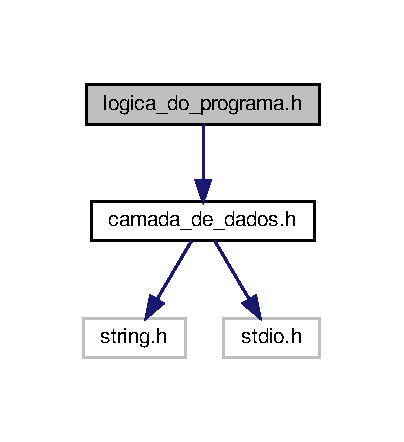
\includegraphics[width=194pt]{logica__do__programa_8h__incl}
\end{center}
\end{figure}
This graph shows which files directly or indirectly include this file\+:
\nopagebreak
\begin{figure}[H]
\begin{center}
\leavevmode
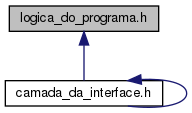
\includegraphics[width=216pt]{logica__do__programa_8h__dep__incl}
\end{center}
\end{figure}
\subsection*{Functions}
\begin{DoxyCompactItemize}
\item 
\mbox{\Hypertarget{logica__do__programa_8h_aa302374c28d47481589def1bbb75eed7}\label{logica__do__programa_8h_aa302374c28d47481589def1bbb75eed7}} 
int \hyperlink{logica__do__programa_8h_aa302374c28d47481589def1bbb75eed7}{casa\+\_\+vencedora} (\hyperlink{structESTADO}{E\+S\+T\+A\+DO} $\ast$e, \hyperlink{structCOORDENADA}{C\+O\+O\+R\+D\+E\+N\+A\+DA} c)
\begin{DoxyCompactList}\small\item\em Função que se o jogo acabou. \end{DoxyCompactList}\item 
\mbox{\Hypertarget{logica__do__programa_8h_acd1b2f5c71c17e023af74e3c678029a9}\label{logica__do__programa_8h_acd1b2f5c71c17e023af74e3c678029a9}} 
int \hyperlink{logica__do__programa_8h_acd1b2f5c71c17e023af74e3c678029a9}{jogada\+\_\+e\+\_\+valida} (\hyperlink{structESTADO}{E\+S\+T\+A\+DO} $\ast$estado, \hyperlink{structCOORDENADA}{C\+O\+O\+R\+D\+E\+N\+A\+DA} c)
\begin{DoxyCompactList}\small\item\em Função que verifica se uma jogada é possivel. \end{DoxyCompactList}\item 
\mbox{\Hypertarget{logica__do__programa_8h_a53472e75f056ceb02b5387193021838a}\label{logica__do__programa_8h_a53472e75f056ceb02b5387193021838a}} 
int \hyperlink{logica__do__programa_8h_a53472e75f056ceb02b5387193021838a}{jogar} (\hyperlink{structESTADO}{E\+S\+T\+A\+DO} $\ast$estado, \hyperlink{structCOORDENADA}{C\+O\+O\+R\+D\+E\+N\+A\+DA} c)
\begin{DoxyCompactList}\small\item\em Função que altera o estado do jogo através das coordenadas fornecidas. \end{DoxyCompactList}\end{DoxyCompactItemize}


\subsection{Detailed Description}
Definição das funções da componente lógica do jogo 
\hypertarget{main_8c}{}\section{main.\+c File Reference}
\label{main_8c}\index{main.\+c@{main.\+c}}
{\ttfamily \#include $<$stdio.\+h$>$}\newline
{\ttfamily \#include $<$string.\+h$>$}\newline
{\ttfamily \#include \char`\"{}camada de dados.\+h\char`\"{}}\newline
{\ttfamily \#include \char`\"{}camada da interface.\+h\char`\"{}}\newline
{\ttfamily \#include \char`\"{}logica do programa.\+h\char`\"{}}\newline
Include dependency graph for main.\+c\+:
\nopagebreak
\begin{figure}[H]
\begin{center}
\leavevmode
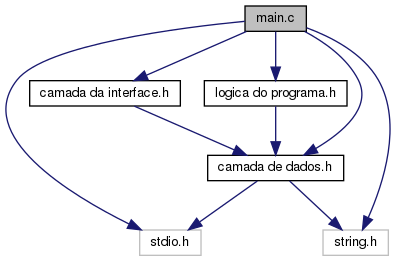
\includegraphics[width=305pt]{main_8c__incl}
\end{center}
\end{figure}
\subsection*{Functions}
\begin{DoxyCompactItemize}
\item 
\mbox{\Hypertarget{main_8c_ae66f6b31b5ad750f1fe042a706a4e3d4}\label{main_8c_ae66f6b31b5ad750f1fe042a706a4e3d4}} 
int \hyperlink{main_8c_ae66f6b31b5ad750f1fe042a706a4e3d4}{main} ()
\begin{DoxyCompactList}\small\item\em Função principal que aglomera todos os módulos. \end{DoxyCompactList}\end{DoxyCompactItemize}


\subsection{Detailed Description}
Aglomeração de todas as camadas 
%--- End generated contents ---

% Index
\backmatter
\newpage
\phantomsection
\clearemptydoublepage
\addcontentsline{toc}{chapter}{Index}
\printindex

\end{document}
